\section{Ocean Dataset and Validation}
\label{app:data}

\subsection{Sources, harmonization, and schema}

OneOcean combines bathymetry from the General Bathymetric Chart of the Oceans (GEBCO) \cite{GEBCO2025} with horizontal currents from the Copernicus Marine Service Global Ocean Physics Analysis and Forecast (GOPAF) product \cite{copernicus,CopernicusGOPAF2025}. The resulting Network Common Data Form (NetCDF) product is harmonized by cropping the requested region, retaining returned time and depth coordinates, normalizing coordinate names and units, interpolating variables onto one latitude--longitude grid, preserving invalid terrain and NoData cells, and recording the transformations.

\begin{figure*}[t]
\centering
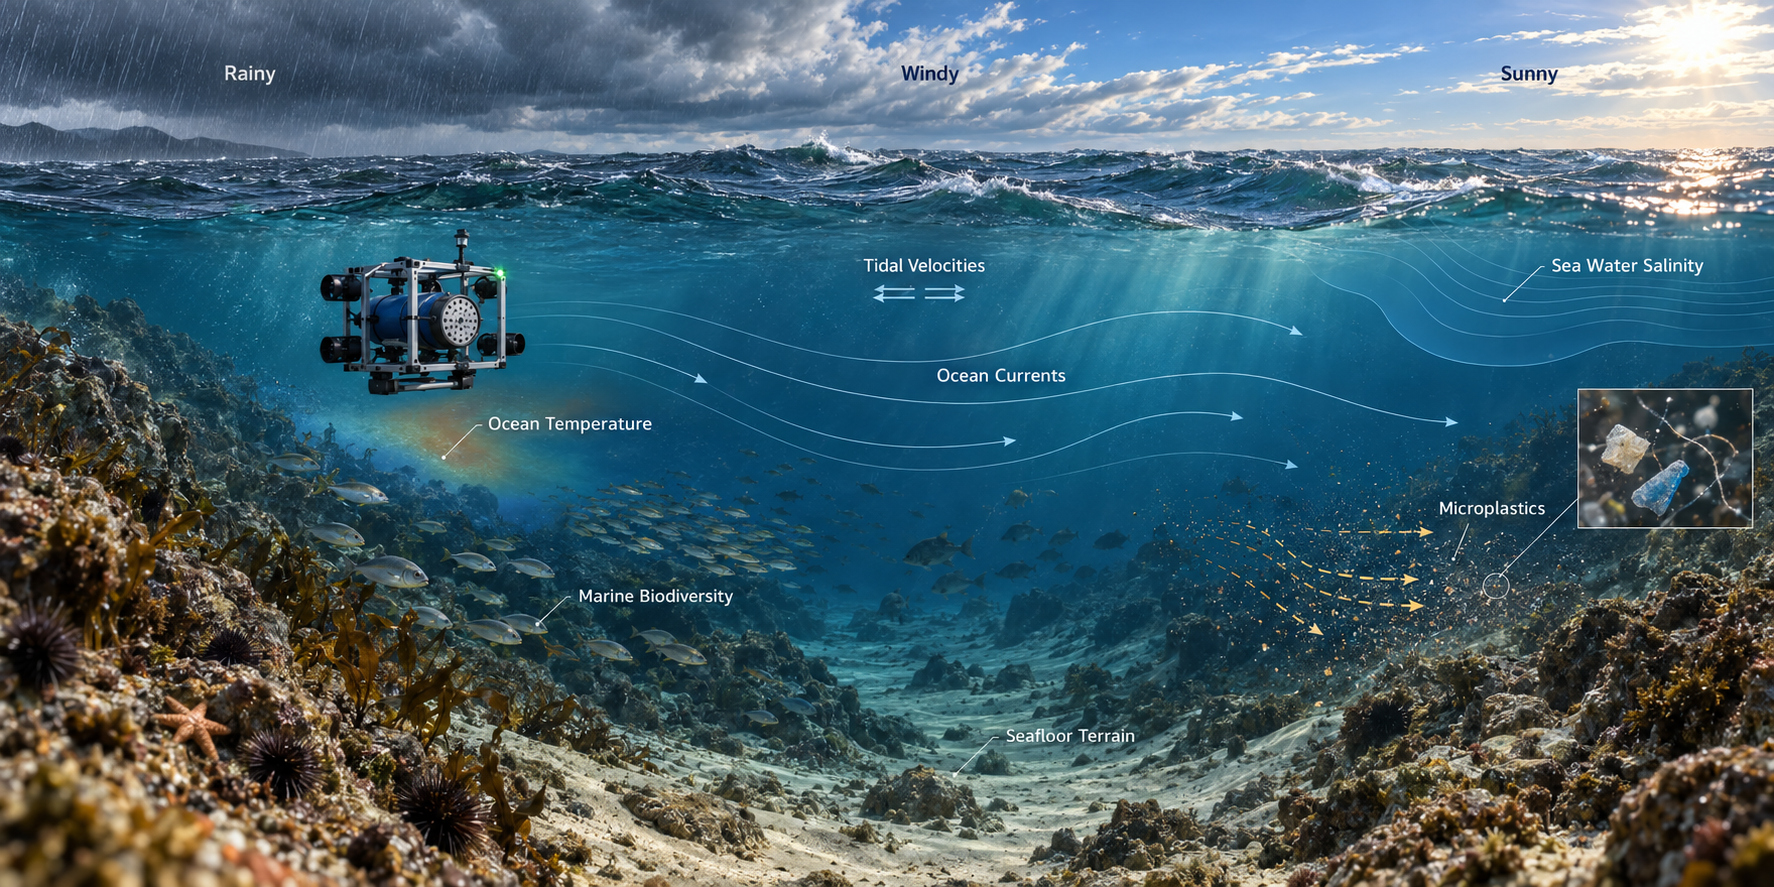
\includegraphics[width=0.98\textwidth]{figures/overview2.jpg}
\caption{Conceptual overview of ocean conditions and ecological signals relevant to OneOcean, including terrain, currents, tides, temperature, salinity, weather, biodiversity, and microplastics.}
\label{fig:app_environment_overview}
\end{figure*}

\begin{table*}[t]
\centering
\scriptsize
\setlength{\tabcolsep}{4pt}
\renewcommand{\arraystretch}{1.10}
\begin{tabularx}{\textwidth}{l l l X}
\toprule
\textbf{Canonical field} & \textbf{Dimensions} & \textbf{Unit or Encoding} & \textbf{Contract} \\
\midrule
Latitude & $H$ & degrees north & Strictly monotonic geographic coordinate. \\
Longitude & $W$ & degrees east & Strictly monotonic geographic coordinate. \\
Time & $T$ & Climate and Forecast time unit & Monotonic timestamps retained from the source product. \\
Depth & $D$ & m, positive down & Actual depth coordinates returned by the source. \\
Eastward and northward current & $T\!\times\!D\!\times\!H\!\times\!W$ & m\,s$^{-1}$ & Base pair $(u,v)$ or tide-combined pair $(u_{\mathrm{total}},v_{\mathrm{total}})$. \\
Elevation & $H\!\times\!W$ & m relative to sea surface & Bathymetric elevation aligned to the current grid. \\
Validity mask & $H\!\times\!W$ & binary & Invalid terrain, crop-exterior, or NoData cells. \\
\bottomrule
\end{tabularx}
\caption{Canonical environment-product schema. The validator accepts documented aliases but maps every accepted product to these semantics.}
\label{tab:app_data_contract}
\end{table*}

Masked elevation cells use zero as a storage fill value; elevation is interpreted together with the validity mask. In the core simulation frame, $(x,y,z)=$(east, depth-down, north), and the dataset vector $(u,v)$ maps to $(u,0,v)$. Longitude and latitude are converted to local metric $x$ and $z$ about the recorded lower-left geographic origin.

\subsection{Depth and tide treatment}

The realized \texttt{tiny} request contains one level at 0.494\,m. The \texttt{scene} and \texttt{public} requests cover 0--200\,m and retain 26 source levels from 0.494 to 186.126\,m. The pipeline retains the returned depth coordinates. Consequently, \texttt{tiny} is a time-varying 2D or 2.5D current product, whereas the other two products provide source-derived horizontal current at multiple discrete depths.

Only the current \texttt{scene} release includes tide components. Hourly tide samples are aligned to the base product with nearest-time selection and attenuated as $\exp(-d/z_0)$ with $z_0=50$\,m before forming the total current pair. The exported temporal resolution follows the base-product clock; coarse time sampling removes higher-frequency variation.

\subsection{Dataset validation}

The release validator checks required fields, aliases, dimensions, monotonic coordinates, units, finite sampled values, mask semantics, provenance, and optional round-trip fidelity between NetCDF and a NumPy Archive (NPZ). Table~\ref{tab:app_validator} summarizes the July 21, 2026 validation of the released products.

\begin{table}[t]
\centering
\scriptsize
\setlength{\tabcolsep}{3pt}
\renewcommand{\arraystretch}{1.10}
\begin{tabularx}{\columnwidth}{l X c c l}
\toprule
\textbf{Variant} & \textbf{Current pair} & \textbf{Errors} & \textbf{Warn.} & \textbf{Round-trip} \\
\midrule
\texttt{tiny} & \texttt{uo}, \texttt{vo} & 0 & 3 & Exact \\
\texttt{scene} & \texttt{utotal}, \texttt{vtotal} & 0 & 4 & Not run \\
\texttt{public} & \texttt{uo}, \texttt{vo} & 0 & 2 & Not run \\
\bottomrule
\end{tabularx}
\caption{Environment-product validation. All variants are \texttt{PASS\_WITH\_WARNINGS}; the metadata warnings are listed below. Round-trip denotes the fixed \texttt{tiny} $(t=0,d=0)$ NetCDF-to-NPZ check.}
\label{tab:app_validator}
\end{table}

The warnings identify missing depth or elevation units, total-current units, or mask flag meanings depending on the variant. Regeneration with the updated pipeline writes these attributes. The tested \texttt{tiny} slice preserved coordinates and currents at absolute tolerance $10^{-6}$.

\subsection{Portable provenance}

Every regenerated NetCDF records source product identifiers, requested and actual region, time, and depth, tide inclusion and depth profile, interpolation and missing-value handling, and generation software. Companion variant manifests use paths relative to the variant directory. Each run records the selected time and depth indices.

\subsection{Geographic sampling within an episode}

Let $(\phi_0,\lambda_0)$ be an episode's geographic origin and $p=(x,y,z)$ its local position in meters. The core sampler uses
\begin{align}
\phi(p)&=\phi_0+z/L,\\
\lambda(p)&=\lambda_0+x/[L\max(0.1,\cos\phi_0)],
\end{align}
where $L=111132$\,m per degree and the cosine evaluates latitude in radians. At reset, the origin is sampled within the available geographic extent to place the simulation tile on the environmental grid. The default tile spans $600\times600$\,m horizontally, with vehicle depth bounded between 2 and 18\,m. Environmental coordinates retain the source grid spacing.

For grid coordinates $\{\phi_j\}$ and $\{\lambda_k\}$, the sampled indices are
\begin{equation}
j^*=\arg\min_j|\phi_j-\phi(p)|,\qquad
k^*=\arg\min_k|\lambda_k-\lambda(p)|.
\end{equation}
The current at $p$ is $g(u_{j^*k^*},0,v_{j^*k^*})$, where $g$ is the current gain. Bathymetry and validity use the same indices. Missing current samples are set to zero, while terrain feasibility is determined separately by the validity mask and seabed clearance. Core episodes query a fixed time and depth slice.

\subsection{Temporal forcing in the scene backend}

The scene backend uses an exported current sequence at a selected geographic location and the nearest available source depth. Let $T_c$ be its number of temporal samples, $s$ the episode seed, and $\alpha$ the configured sequence-advance rate. At simulation time $t$, the sampled index is
\begin{equation}
i(t)=\big[(s\bmod T_c)+\lfloor\alpha t\rfloor\big]\bmod T_c.
\end{equation}
Setting $\alpha=0$ holds the initial sample; a positive value advances the sequence and wraps at its end. For a daily export, $\alpha$ gives source days per simulated second. The sampled vector, multiplied by the current gain, drives the scene disturbance. Spatial slices and temporal sequences provide complementary conditions for evaluating disturbance rejection.
